% Section 7: Results

\section{Results}

\subsection{Summary of Runs}

Much as with DC2, we executed numerous but short pipeline runs over
a sampling of the data from the CFHT-LS fields D3 and D4 and from the
simulated data collections, SimDeep and SimWide.  These short runs
were used to do initial debugging, performance analysis, and quality
analysis which resulted in numerous bug fixes and important algorithm
optimizations.  These short runs also allowed to explore different
policy parameter settings to understand the trade off between data
quality and performance.  

For our final, detailed analysis of the data quality and processing
performance, we focused on two productions runs with identical
versions of the software and configuration: {\tt rlp1233} and {\tt
rlp1234}.  As summarized in Table \ref{T7-1}.  These two runs
processed different subsets of the focal plane for 85 visits to the
CFHT-LS D3 on our own LSST cluster.  These visit were selected based
on the availability of the calibration data needed to calibrate raw
science images.  The Image Processing and Source Detection (IPSD)
pipeline featured 1 master pipeline and 31 slice processes running
across four nodes of the cluster (thus each run processed 31 amplifier
images in parallel).  The Association pipeline (ap) ran on node 10
within one master process and one slice process.  The ``NightMOPS''
pipeline (part of the Moving Objects Prediction System) ran on node 9
with 1 master process and 5 slice processes.  Taking a lesson from
DC2, we did not use any of the ``slower'' cluster nodes (nodes 1-4)
for pipeline processes as they would have pulled down the over
performance of the pipeline.  We note that we had other infrastructure
processes on the cluster nodes running which did not interfere
noticeably with the pipeline processes.  Node 4 (which did not have
any pipeline processes on it) hosted the event broker process, and
node 9 (which had extra unused processor cores available) hosted the
event monitor which loaded logging events into the database.

One of the intended goals of the DC3a was exercise the use of the
parallel filesystem, Lustre, we installed on the LSST cluster.  Much
as with DC2, we found Lustre to be fairly unstable under heavy IO,
apparently causing catastrophic failure of the filesystem.  This may
have been due to an insufficient number of fileserver nodes for the
level of IO we were attempting; however, schedule and hardware
resource limitations prevented our exploring the causes in any
detail.  Consequently, the final runs were conducted using NFS-mounted
filesystems (which are known to perform poorly most conditions).  

Ultimately, the simulated data was not used as part of the final
analysis.  While the two simulated collections were instrumental
in understanding and correcting processing problems, we found that the
quality of the template images were insufficient for producing useful
difference images and database results.  

In addition to the runs on our own LSST cluster, we also conducted
runs on the NCSA Abe cluster.  The purpose of these runs were to
explore the scalability of the pipeline processing up to higher
numbers of slices.  In particular, we have executed runs that process
entire CFHT focal plane exposures simultaneously.  This was done by
running the IPSD pipeline on Abe with 288 slice processes across 36
8-core nodes.  While Image I/O was carried out using the Lustre
filesystem attached to that platform, database I/O occurred with the
database residing on the LSST cluster ({\tt lsst10}).  

DC3a schedule constraints limited the detailed analysis
that could be completed for this report; nevertheless, we see that the
pipeline scaled fairly well at this level.  One critical barrier to
scaling, however, was in the event broker (powered by the
third-party product, activemq), which failed while processing the
thirteenth visit which in turn disabled the pipelines.  The reasons
are unclear; though, it appears to be due to the total volume of
events processed rather than the rate of at which the events were
generated.  

These Abe runs provided additional qualitative accomplishments:

\begin{itemize}
\item they revealed configurable system limits that must be increased:
\begin{itemize}
\item the event broker must support over 1000 simultaneous open file
  descriptors 
\item the MySQL database must support $\gtrsim$ 300 simultaneous
  connections.  
\end{itemize}
\item we demonstrated the integration of grid-based job management
  (via Condor-g) into our orchestration layer
\item we demonstrated the successful use of the parallel Lustre
  filesystem.  
\end{itemize}

\noindent Additional information about the results of these runs on
Abe can be found in section \ref{sec:timing}.  

Table \ref{tbl:runsummary} summarizes the pertinent production runs
referenced in this section.

\begin{table}[htbp]
\centering
\caption{Average Processing Times Per Visit
\label{tbl:runsummary}}
\vspace{\baselineskip}
\begin{tabular}{ | r | r | r | r | r | r |}
\hline\hline
runId & nVisits & nAmps & inputImages & outputImages & outputFrac \\ \hline
rlp1233 & 85  & 31 &  &  &  \\ \hline
rlp1234 & 85  & 31 &  &  &  \\ \hline
rlpabe041 & 12  & 288 &  &  &  \\ \hline
Total   & --- &    &  &  &  \\ \hline
\end{tabular}
\end{table}

\subsection{Science Data Quality}

\subsection{Timing Results}
\label{sec:timing}

As in DC2, we use the logging framework (in which every log message is
time-stamped) to instrument our pipeline processing code.  We can
calculate how much time is spent on the different contributors to the
overall processing time, including I/O, middleware overhead,
scientific processing.  

\begin{table}[htbp]
\begin{center}
\caption{Average Processing Times Per Visit
\label{tbl:visitstats}}
\vspace{\baselineskip}
\begin{tabular}{ l | c | c |}
\hline\hline
          & Total Processing Time, corrected
          & Application Processing Time \\ 
Pipeline  & average $\pm$  $3\sigma$ (s) & average $\pm$ $3\sigma$ (s) \\ \hline
IPSD      & 264.7 $\pm$ 20.2 & 264.1 $\pm$ 20.1  \\ 
nightmops & 10.6  $\pm$  4.4 & 0.174 $\pm$  4.4  \\ 
ap        & 1.4   $\pm$  0.7 & 0.021 $\pm$  0.7  \\ \hline
\hline
\end{tabular}

\end{center}
\end{table}

In table \ref{tbl:visitstats}, we summarize the statistics for processing
a single visit through each pipeline.  For each quantity, the error
given represents the calculated $3\sigma$ variation of the
distribution of values.  The total time is corrected to remove the
time the pipelines spend waiting for data events to arrive.  For the
IPSD and nightmops pipelines, this is the time it waits for a new data
event to arrive.  As mentioned in section \ref{brokerprob}, we
throttled the time between to data events to match the expected visit
nnprocessing time to avoid having too many unconsumed data events pile
up in the event broker; this typically resulted in an extra 20-30
second wait for a data event before processing could resume.  The ap
pipeline, on the other hand, receives its initial event from the IPSD
pipeline; thus, it had to wait on average 4.4 minutes for the IPSD
pipeline to complete before it could do its work.

\begin{figure}[hb]
\begin{center}
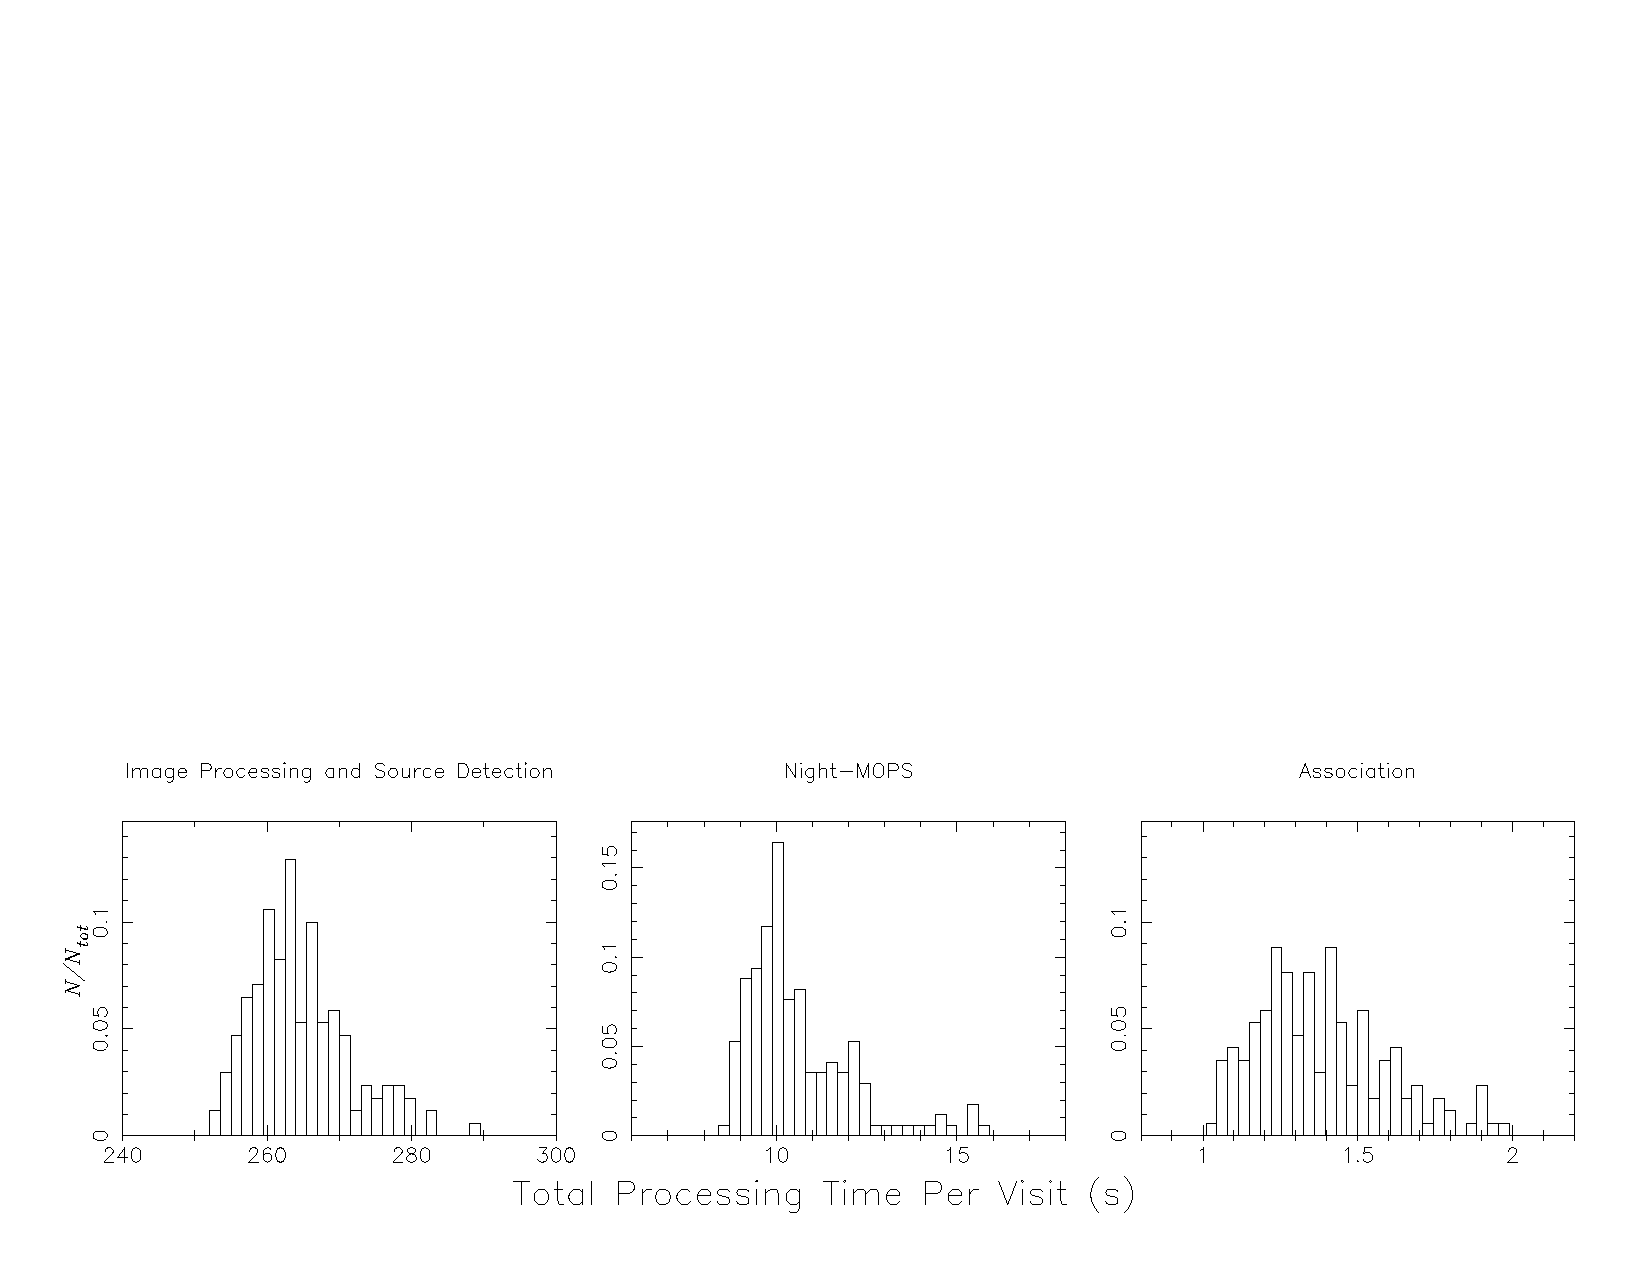
\includegraphics[width=\textwidth,bb=0 0 800 276,viewport=25 25 775 250,clip]{images/visitdist.pdf}
\caption{Histogram of the times to process each visit (not including
  time waiting on data events).  The $y$-axis measure the fraction of
  the 170 visits in each time bin.  
\label{fig:visitdist}}
\end{center}
\end{figure}


The ``Application Processing Time'' tallies on the time spent in total
by all the pipeline stages in their preprocess, process, and
postprocess functions where I/O is carried out and application
algorithms are applied.  (The times in these functions are included
only in cases where a stage actually provides an implementations for
them.)  It excludes the overhead by the pipeline framework for
managing the execution of the stages.  As the numbers show, the
pipeline adds very little to the processing time of a visit.  A more
precise analysis of the pipeline overhead is presented below.  

The variation in the processing is in general much smaller in DC3a as
it was in DC2: in the latter, the $3\sigma$ half-width was 108
seconds in the image processing pipeline, while we now have 20
seconds.  Furthermore as illustrated in Fig. \ref{fig:visitdist}, the
processing times do not feature the unexplained double-peaked
distributions we saw in DC2.  In summary, our we're getting much more
consistent processing times in DC3a than we did in DC2.  This has an
important impact on the overall performance because the total time
spent on a stage is driven primarily by the duration of the slice that
took the longest time.  

Tables \ref{tbl:ipsdstages} and \ref{tbl:otherstages} list the average
time spent in actual {\it application code} each stage for each pipeline.
(That is, these include the time spent in the {\tt preprocess()}, 
{\tt process()}, and {\tt postprocess()} functions only when these
were provided by a stage implementation.)  The type (``tp'') column
differentiates between stages that handle I/O and those that only
apply a scientific algorithm to the data.  

\begin{table}[p]
\begin{center}
\small
\caption{IPSD: Average Processing Times (s) Per Stage for {\tt rlp1233, rlp1234}
\label{tbl:ipsdstages}}
\vspace{\baselineskip}
\begin{tabular}{lrlrr}
\hline\hline
\# & tp & Name & \multicolumn{1}{c}{average}&\multicolumn{1}{c}{$3\sigma$} \\ 
\hline
 1 &    &                     sliceInfo &  0.002 &  0.001 \\
 2 &    &                       symLink &  0.001 &  0.001 \\
 3 &  I &                   imageInput0 &  1.804 &  0.527 \\
 4 & *\phantom{I} &                visitMetadata0 &  0.076 &  0.975 \\
 5 &    &            transformMetadata0 &  0.013 &  0.007 \\
 6 &    &             validateMetadata0 &  0.002 &  0.001 \\
 7 &  I &          visitMetadataOutput0 &  0.001 &  0.001 \\
 8 &  I &    rawImageAndMetadataOutput0 &  1.999 &  0.374 \\
 9 & *\phantom{I}  &   identifyCalibrationProducts &  0.020 &  0.008 \\
10 & *I &              calibrationInput & 11.927 &  2.810 \\
11 &    &  transformCalibrationMetadata &  0.004 &  0.003 \\
12 & *S &                          isr0 &  1.604 &  0.135 \\
13 & *S &               sourceDetection &  1.685 &  0.449 \\
14 &  I &    calibAndBkgdExposureOutput & 10.627 &  1.536 \\
15 &  S &             sourceMeasurement &  1.093 &  2.028 \\
16 & *I &   exposureAndWcsSourcesOutput &  0.228 &  0.245 \\
17 & *S &              psfDetermination &  0.207 &  0.149 \\
18 &  I &                     psfOutput &  0.120 &  0.097 \\
19 &  I &                   imageInput1 &  1.761 &  0.494 \\
20 &    &                visitMetadata1 &  0.038 &  0.033 \\
21 &    &            transformMetadata1 &  0.013 &  0.005 \\
22 &    &             validateMetadata1 &  0.002 &  0.002 \\
23 &  I &          visitMetadataOutput1 &  0.002 &  0.002 \\
24 &  I &    rawImageAndMetadataOutput1 &  2.126 &  0.553 \\
25 & *S &                          isr1 &  1.709 &  0.466 \\
26 & *I &               wcsSourcesInput &  0.034 &  0.029 \\
27 & *S &              wcsDetermination &  0.194 &  0.050 \\
28 & *I &     calibratedExposuresOutput & 10.514 &  1.819 \\
29 & *\phantom{I}  &              CcdMetadataStage &  0.002 &  0.001 \\
30 & *I &         templateMetadataInput &  0.062 &  0.089 \\
31 & *\phantom{I}  &             templateDimension &  0.016 &  0.005 \\
32 & *\phantom{I}  &                  templateBBox &  0.004 &  0.001 \\
33 & *I &         templateSubimageInput & 27.218 &  3.925 \\
34 &  I &        templateSubimageOutput &  5.574 &  1.043 \\
35 & *S &              imageDifference0 & 82.343 &  9.706 \\
36 & *S &              imageDifference1 & 80.247 & 11.998 \\
37 & *I &         differenceImageOutput & 10.172 &  1.606 \\
38 & *S &                  addAndDetect &  7.966 &  0.126 \\
39 & *S &          diaSourceMeasurement &  0.473 &  2.211 \\
40 & *\phantom{I}  &             sourceToDiaSource &  0.050 &  0.082 \\
41 & *S &          sourceClassification &  0.008 &  0.007 \\
42 & *I &              diaSourceOutput0 &  1.947 &  4.220 \\
43 & *I &              diaSourceOutput1 &  0.106 &  0.143 \\
44 & *\phantom{I}  &              associationEvent &  0.002 &  0.001 \\
45 & *I &                   sdqaOutput0 &  0.047 &  0.015 \\
46 & *I &                   sdqaOutput1 &  0.028 &  0.010 \\
\hline
\multicolumn{5}{l}{Type codes: I = input/output stage, * = production stage,} \\
\multicolumn{5}{l}{S = Stage applying a scientific algorithm} \\
\end{tabular}
\end{center}
\end{table}

As in DC2, the costliest stages are those that do image subraction
(stages 35 and 36) at 80 seconds per image.  This is down
significantly from DC2's 175 seconds; although, in DC3 we now do image
subtraction on both exposures from a visit.  The variation in the time
is down considerably as well.  One of the tunable parameters we found
that can have a significant effect on the subtraction time is the 
{\tt maxPrincipalComponents} policy parameter, which controls the number
of principal components calculated for the ... step and which in this
run was set to 10.  We believe that we can probably reduce this
parameter to 5 without loss in processing fidelity; subsequent tests
with this value ({\tt rlp1248}) indicate that this would reduce the
duration of the image subtraction stage by another 20 seconds.

\begin{table}[p]
\begin{center}
\small
\caption{Night-MOPS and Association: Average Processing Times (s) Per
  Stage for {\tt rlp1233, rlp1234} 
\label{tbl:otherstages}}
\vspace{\baselineskip}
\begin{tabular}{lrlrr|lrlrr}
\hline\hline
\multicolumn{5}{c|}{Association} & \multicolumn{5}{c}{Night-MOPS} \\
\# & tp & Name & \multicolumn{1}{c}{average}&\multicolumn{1}{c|}{$3\sigma$} &
\# & tp & Name & \multicolumn{1}{c}{average}&\multicolumn{1}{c}{$3\sigma$} \\ 
\hline
1 &    & symLink                  &  0.001 &  0.006 & 1 & *S & NightMopsStage           & 10.228 &  4.485 \\ 
2 &  I & load                     &  0.458 &  0.081 & 2 & *I & output                   &  0.155 &  0.597 \\ 
3 & *I & diaSourceInput           &  0.015 &  0.017 & 3 & *\phantom{I}  & associationEvent         &  0.020 &  0.078 \\ 
4 & *S & MatchDiaSourcesStage     &  0.005 &  0.005 &&&&&\\ 
5 & *S & diaSourceMatchOutput     &  0.259 &  0.406 &&&&&\\ 
6 & *I & predInput                &  0.003 &  0.004 &&&&&\\ 
7 & *S & MatchMopsPredsStage      &  0.002 &  0.002 &&&&&\\ 
8 & *I & predMatchAndObjectOutput &  0.112 &  0.231 &&&&&\\ 
9 & *I & store                    &  0.379 &  0.248 &&&&&\\ 
\hline
\multicolumn{10}{l}{Type codes: I = input/output stage, S = Stage
  applying a scientific algorithm, * = production stage,} \\
\multicolumn{5}{l}{} \\
\end{tabular}
\end{center}
\end{table}

